%!TEX root = LiteratureReview.tex

\section{Breakdown of Photon Blockade: A Dissipative Quantum Phase Transition in Zero Dimensions}
The driven Jaynes Cumming oscillator exhibits a characteristic Kerr nonlinearity ($n \propto I$) under strong coherent drive, called \emph{photon blockade}\autocite{Carmichael2015}. The author presents conditions for breakdown of photon blockade through increasing drive strength, and characterises the corresponding dissipative quantum phase transition, and further numerical simulations highlight the differences between quantum and semiclassical approaches.
\subsection{Photon Blockade}
With the cavity field on resonance ($\omega_A = \omega$) with the two level transition, the JC Hamiltonian~\cref{HJC} can be written\autocite[3]{Carmichael2015}
\begin{equation}
  \ham_{JC} = \hbar \omega (\cre \ann + \atann \atcre) +\hbar g (\cre \atann + \hat{a} \atcre)
\end{equation}
after a rescaling the atomic energy levels. Diagonalising yields the \emph{dressed states}
\begin{align}
  \ket{E_{n, U}} & = \frac{1}{\sqrt{2}} (\kettens{n}{-}+\kettens{n-1}{+}) \\
  \ket{E_{n, L}} & = \frac{1}{\sqrt{2}} (\kettens{n}{-}-\kettens{n-1}{+})
\end{align}
in the tensor product of the field fock space and the atomic eigenspace spanned by $\ket{+}, \ket{-}$. These eigenstates are superpositions of the bare states $\kettens{n}{-}$ and $\kettens{n-1}{+}$ and are balanced only in the case of zero detuning, which we consider here. The eigenenergies are
\begin{align}
  E_{n, U} &= n \hbar \omega_0 + \sqrt{n} \hbar g \\
  E_{n, L} &= n \hbar \omega_0 - \sqrt{n} \hbar g
\end{align}
in which the Rabi splitting between the upper and lower dressed states is clear. In the absence of coupling to a dressing field $(g=0)$ the Jaynes-Cumming energies form a degenerate harmonic ladder; considering coupling to the cavity field induces an anharmonicity via the characteristic $\sqrt{n}$ Rabi splitting.

We now consider the effect of an external drive tuned to the $\ket{G} \rightarrow \ket{E_{1, U/L}}$ transition\footnote{Drive frequencies at multiphoton resonances induce the same effect} (where $\ket{G}$ is the coincident dressed ground state $\ket{E_{0, -}} = \kettens{0}{-}$) with frequency $\omega_D = \hbar \omega_0 \pm \hbar g$.
The $\kettens{1}{U/L} \rightarrow \kettens{2}{U/L}$ step of the Jaynes Cummings ladder is now detuned from the drive by $E_{2, U/L} - E_{1, U/L} - \hbar \omega_D =  \mp(2-\sqrt{2}) \hbar g$. Thus for sufficiently large g and sufficiently small linewidth, the upper steps of the ladder are inaccessible, and the Jaynes Cumming system behaves as a two-level system until the photon is reemitted through some loss process. This is the photon blockade effect.
\subsubsection{Large n detuning approximation}
Given a driving field as above, the upper and lower path rungs (n, n+1, \dots) will be detuned
\begin{align}
  \Delta E_u = \hbar g (\sqrt{n}-\sqrt{n-1}) \\
  \Delta E_l = -\hbar g (\sqrt{n}-\sqrt{n-1})
\end{align}
approximated for large n by
\begin{align}
  \Delta E_u &= \hbar g \sqrt{n} \left (1-\sqrt{\frac{n-1}{n}} \right ) \\
  &= \hbar g \sqrt{n} \left (1-\sqrt{1-\frac{1}{n}} \right ) \\
  & \approx \hbar g \sqrt{n} \left ( 1- \left ( 1 - \frac{1}{2n} \right ) \right ) \\
  &= \frac{\hbar g}{2 \sqrt{n}}
\end{align}
and
\begin{equation}
  \Delta E_l = -\frac{\hbar g}{2 \sqrt{n}}
\end{equation}
\subsection{Quantum, Coherent Driving}
The author now considers the Jaynes Cummings oscillator driven by a coherent field. Transformed to an interaction picture, the Hamiltonian for the driven cavity mode\footnote{The driven qubit can be recovered via a transformation \autocite{Alsing1999}} is
\begin{equation}
  \ham_{JC}^{int} = -\hbar \Delta (\cre \ann + \atcre \atann) + \hbar g(\ann \atcre + \cre \atann) + \hbar \Epsilon(\ann + \cre)
\end{equation}
with $\Epsilon$ the coherent state intensity and
\begin{equation}
  \Delta \omega = \omega_D - \omega
\end{equation}
the drive detuning

The Hamiltonian is diagonalised via a Bogliubov transformation\footnote{A Bogliubov transformation is a transformation from one unitary representation to another that is also an isomorphism between the representations' canonical commutator algebras}. The resulting quasi-energy spectrum
\begin{align}
  e_{n, +} &= + \sqrt{n} \hbar g {\left \{1 - {\left ({\frac{2\Epsilon}{g}} \right )}^2 \right \}}^{\frac{3}{4}} \\
  e_{n, -} &= - \sqrt{n} \hbar g {\left \{1 - {\left ({\frac{2\Epsilon}{g}} \right )}^2 \right \}}^{\frac{3}{4}}
\end{align}
A critical point (corresponding to quantum phase transition) appears at $\frac{2\Epsilon}{g} = 1$, where the quasienergy splitting collapses to zero.
\subsection{The Semiclassical Approach}

The author now demonstrates the existence of the same critical point in a semiclassical treatment of the system based on what he calls the neoclassical equations, but are more commonly known as the Maxwell-Bloch equations,
\begin{align}
  &\frac{d \alpha}{dt} = -(\kappa -i \Delta \omega) \alpha-ig \beta \label{eq:alpha}\\
  &\frac{d \beta}{dt} = i \Delta \omega \beta +ig \alpha \zeta \label{eq:beta}\\
  &\frac{d \zeta}{dt} = 2 i g(\alpha^* \beta -\alpha \beta^*)\label{eq:zeta}
\end{align}
With $\kappa$ the cavity loss rate. Since the length of the pseudo-spin is conserved in the absence of loss we have also a fourth equation
\begin{equation}
  4|\beta|^2+\zeta^2 = 1 \label{eq:pseudospin}
\end{equation}
\subsubsection{Neoclassical Radiation Theory}
In the absence of drive and detuning and with the cavity field derivative set to zero
\begin{align}
  & 0 = -\kappa \alpha - ig \beta \\
  \implies & \alpha = \frac{ig}{\kappa} \beta
\end{align}
in \cref{eq:zeta}
\begin{equation}
  \frac{d \zeta}{dt} = -4 g^2 |\beta|^2
\end{equation}
and from \cref{eq:pseudospin}
\begin{align}
   |\beta|^2 &= (1-\zeta^2)/4 \\
\implies \frac{d \zeta}{dt} &= -\frac{g^2}{\kappa} (1-\zeta^2)
\end{align}
We recover the non exponential decay of neoclassical radiation theory
% \begin{figure}
%   \centering
%   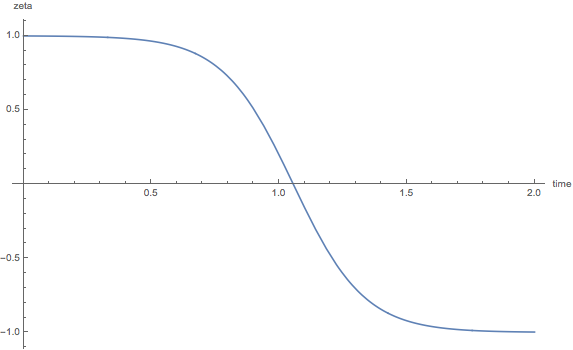
\includegraphics[width=0.5\textwidth]{Images/NeoclassicalDecay.png}
%   \caption{Non-exponential decay of $\zeta$, $\frac{g}{\kappa} = 50, \zeta(0) \approx 1$} \label{fig:neoclassical}
% \end{figure}
\subsubsection{Critical Point}
We consider the equations in the steady state with the field adiabatically eliminated and the detuning zero, after which remain:
\begin{align}
  -ig \beta -i \Epsilon &= 0 \\
  ig\alpha \zeta &= 0
\end{align}
from which two branches of solutions are seen $\rightarrow \zeta = 0$ or $\alpha = 0$. We take $\alpha = 0$ and from \cref{eq:alpha} and \cref{eq:pseudospin}
\begin{align}
  \beta &= -\frac{\Epsilon}{g} \\
  \zeta &= \mp \sqrt{1 - {\left( \frac{2\Epsilon}{g} \right)}^2}
\end{align}
Increasing drive through the critical point $\Epsilon = \frac{g}{2}$ the difference under the square root becomes negative and the inversion $\zeta$ imaginary and unphysical. We take up the other branch $\zeta = 0$, and from \cref{eq:alpha}
\begin{align}
  \beta &= \pm \frac{\alpha}{2|\alpha|} \\
  \zeta &= 0
\end{align}
with $\alpha$ a solution to
\begin{equation}
  \alpha = -i \Epsilon{\left ( \kappa \pm i \frac{g}{2|\alpha|} \right )}^{-1}
  \label{eq:alphacondnotdet}
\end{equation}

\begin{figure}[h]
  \begin{minipage}{.5\linewidth}
    \centering
    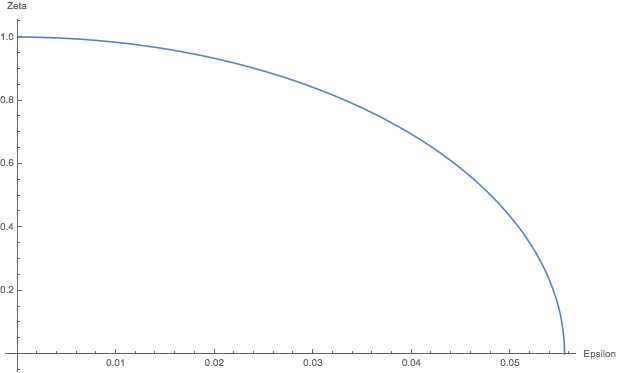
\includegraphics[width=1\textwidth]{Images/MeanFieldBelowCritical.png}
    \subcaption{$\zeta$ approaches zero with increasing drive strength (positive branch)}\label{fig:zeta}
  \end{minipage}%
  \begin{minipage}{.5\linewidth}
    \centering
    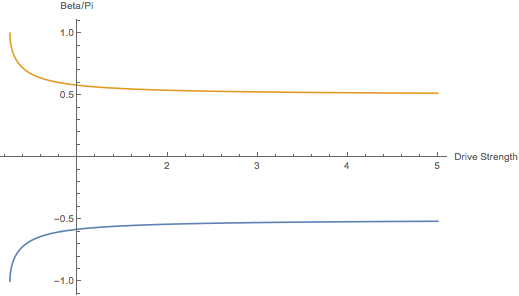
\includegraphics[width=1\textwidth]{Images/MeanFieldAboveCritical.png}
    \subcaption{Phase of $\beta$ with increasing drive greater than critical}\label{fig:alpha}
  \end{minipage}
  \caption{$\alpha$ and $\zeta$ as the drive strength $\Epsilon$ moves up to through and beyond the critical point}
\end{figure}

in \cref{fig:alpha} the phase bistability above the critical point is obvious. The two $\beta$ solution branches start coincident in phase ($\pi$ and $-\pi$) at drive strengths just above critical and quickly move to opposite sides of the Bloch sphere ($-\frac{\pi}{2}$ and $\frac{\pi}{2}$).

The phase of $\beta$ above the critical point follows the phase of $\alpha$, either aligned or antialigned. This spontaneous development of phase bistability Alsing and Carmichael call `Spontaneous Dressed State Polarisation' \autocite{Alsing1999}. Referred to the fully quantum model, each of the two phases corresponds to a the system ascending different sets of rungs of the Jaynes Cummings ladder, either $\ket{E_{n, U}}$ or $\ket{E_{n, L}}$
\subsubsection{Non-zero detuning}
Solving \cref{eq:alpha}, \cref{eq:beta}, \cref{eq:zeta} in the steady state gives
\begin{align}
  \alpha& = i \Epsilon\frac{1}{[\kappa-i(\Delta \omega \mp sgn(\Delta \omega) \frac{g^2}{\sqrt{\Delta \omega^2 +4g^2 |\alpha|^2}})]}
\end{align}
as a condition that $\alpha$ should satisfy, and
\begin{align}
  \beta& = \pm sgn(\Delta \omega) \frac{g \alpha}{\sqrt{\Delta \omega^2 + 4 g^2 |\alpha|^2}}\\
  \zeta& = \mp \sqrt{1-4|\beta|^2}
\end{align}
for $\beta$ and $\zeta$, where $sgn(\Delta \omega)$ is the sign of the detuning with $sgn(0) = 1$.

The expression for $\alpha$ is a Lorentzian, in which is obvious a nonlinear dispersion which diverges as $|\alpha|^2 \rightarrow 0$

A surface plot of $|\alpha|^2 \approx n$ is shown in figure 5b for $\Epsilon>\frac{g}{2}$.
\subsection{Computationally Solving the Master Equation}
\begin{figure}[h]
 \centering
 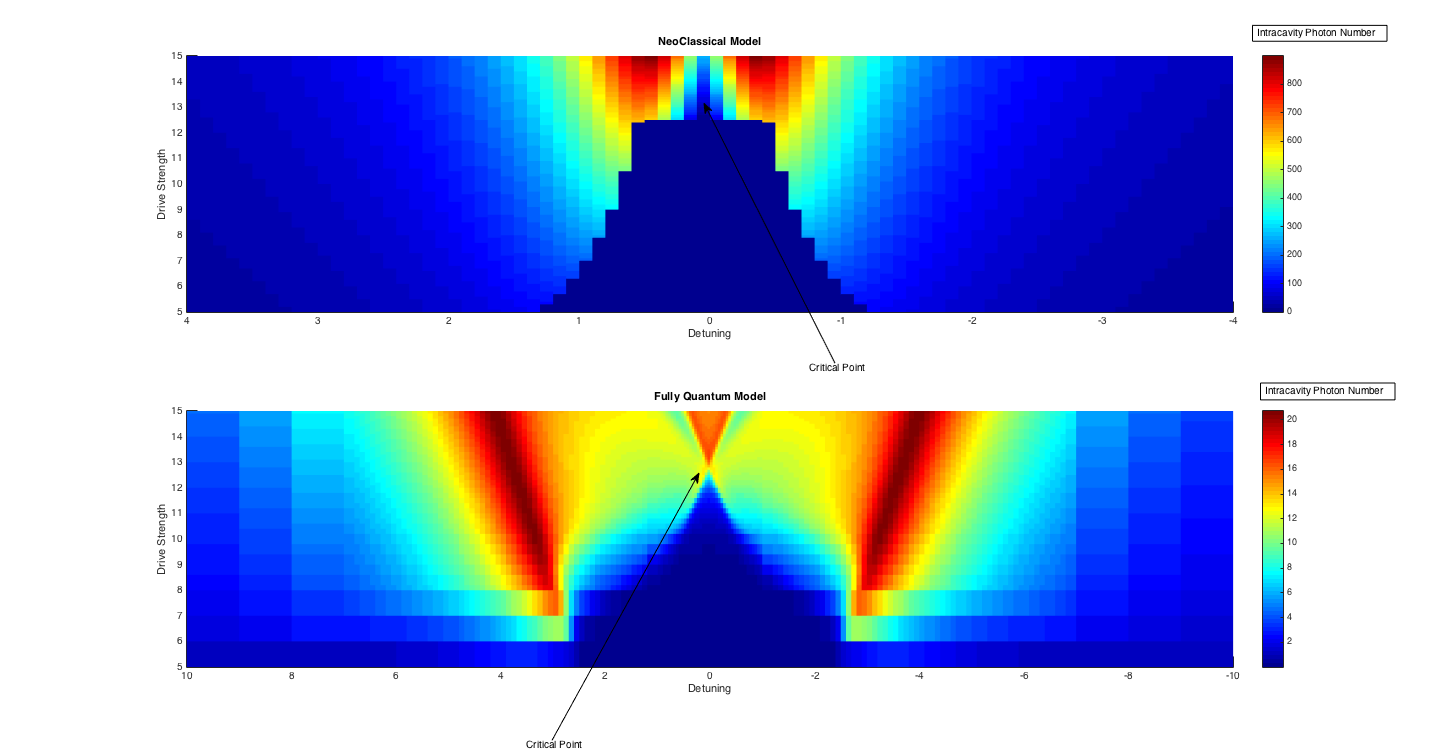
\includegraphics[width=1\textwidth]{Images/MeanFieldvsQuantum.png}
 \caption{Comparison of mean field and fully quantum contour plots with critical points at $\frac{\Epsilon}{2}$ highlighted}\label{fig:MeanFieldvsQuantum}
 \end{figure}


The extension of \autocite{Alsing1999} in this paper is to further classify the fixed point at $\frac{2\Epsilon}{g}$ as an organising centre for the breakdown of the photon blockade phenomenon, which is to say that the fixed point is an attractor in the system phase space.

This is done by truncating the expansion of the density matrix (this is discussed in \autocite{Savage1988}) and solving it using a Runge-Kutta algorithm.The author explains the split Lorentzians in \autocite[Figure 1]{Carmichael2015} via the two distinct Jaynes Cumming ladders and their being climbed by correctly detuned photons. The equal magnitude of each peak is a result of the independence of the two ladders at for high drive strength. Interaction between the ladders via spontaneous emission is treated in \autocite[Section V]{Carmichael2015}

The multiple peaks in the lorentzian (at the bottom of \autocite[Figure 1]{Carmichael2015}) as we move from large to little detuning are a mark of multiphoton blockades and their breaking through.

The author notes the sides of the double lorentzian, most visible in the diagram at the top right of the figure, as domains of coexistence between the near vacuum state and the high occupation state, and the phase transition between the two at this boundary he classifies as first order, in contrast to the transition at the critical point which is second order.

All such features are obvious in the plots in \cref{fig:MeanFieldvsQuantum}, where similar results have been obtained using the steady state master equation solver in the Quantum Optics Toolbox\autocite{qotoolbox}. Computationally solving the for $\alpha$ in the meanfield condition above yields the first plot.

The author then analyses a number of Q function contour plots which show a distinct bimodality. This he uses as an indicator of coexistent states along the aforementioned domain of coexistence. The ratio of the peak heights serves as an estimator of the degree of bistability. He plots a projection of the peak height values onto the system phase space \autocite[Figure 1 right hand side]{Carmichael2015} as \autocite[Figure 2]{Carmichael2015}.

The development of this Q function bimodality is echoed in the Wigner representation, and is clear in \cref{fig:Qbistabilities}, although the parameters are different to those in \cref{fig:MeanFieldvsQuantum} and in \autocite{Carmichael2015}.
\begin{figure}[h]
 \begin{minipage}{.5\linewidth}
  \centering
  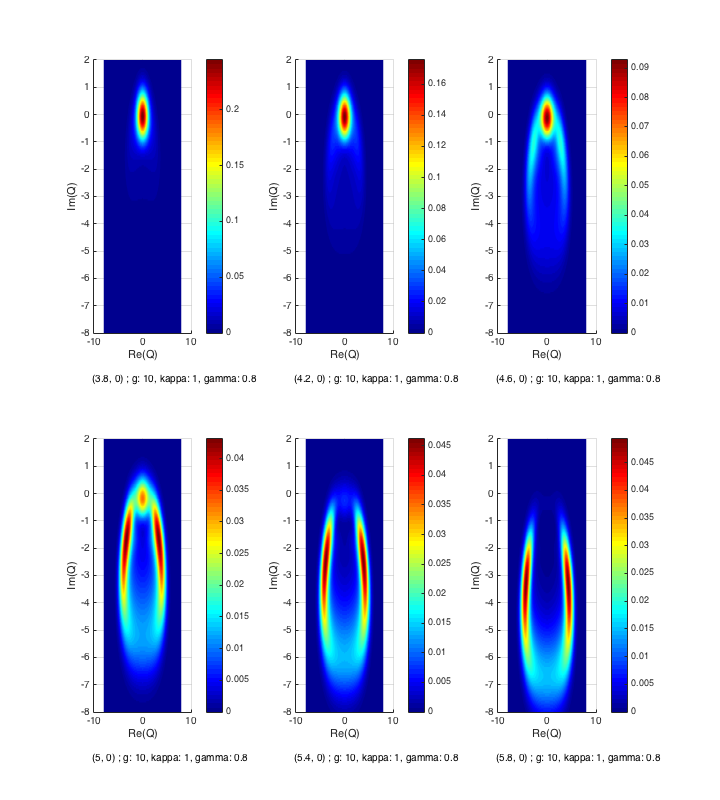
\includegraphics[width=1\textwidth]{Images/Q-Bistability-OnResonance.png}
  \subcaption{Development of phase bistability in the W function for fixed detuning, with drive moving through the critical point at $\frac{\Epsilon}{2}$}
  \end{minipage}%
  \begin{minipage}{.5\linewidth}
      \centering
      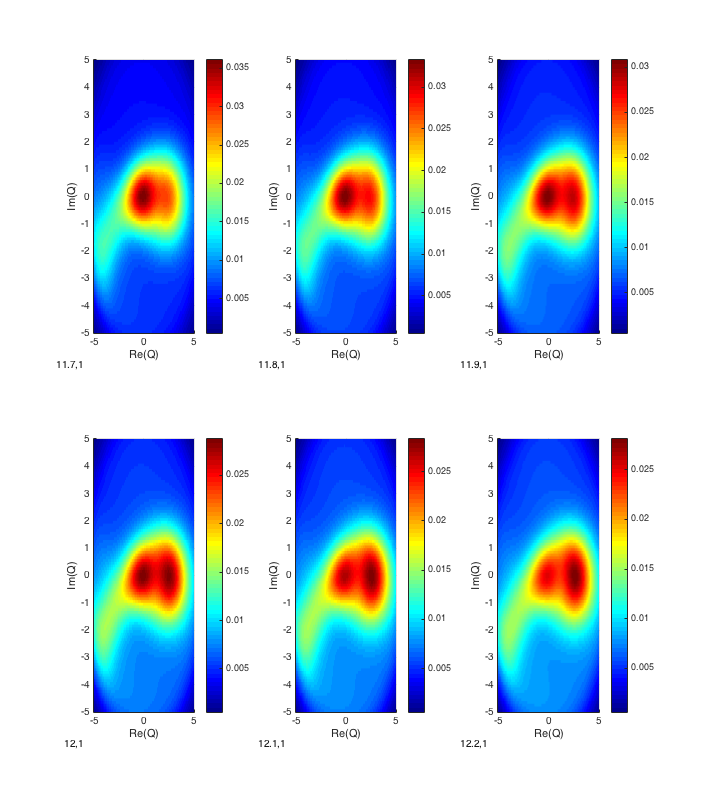
\includegraphics[width=1\textwidth]{Images/Q-Bistability.png}
      \subcaption{W functions with changing detuning and fixed drive. Note the probability fringes to the right connecting the peaks by spontaneous emission}
  \end{minipage}
  \caption{Q-bistabilities}\label{fig:Qbistabilities}
\end{figure}
\subsection{Critical Slowing Down}

A dynamical system perturbed close to an attracting fixed point, towards said fixed point, recovers its equilibrium position more slowly than the same system perturbed further away from the fixed point. This is known as \emph{critical slowing down}\autocite[40, 56]{Strogatz1994}. The author plots in \autocite[Figure 3]{Carmichael2015} two time-dependent photon number curves (green and red) for one point along the domain of coexistence, and one point far from it that show a dramatic critical slowing down in the region of bistability, near to the point $\frac{\Epsilon}{2g} = 1$. This is indicative of the nature of this fixed point: this is an `organising centre', characteristic of a second order transition.

\begin{figure}[h]
  \centering
  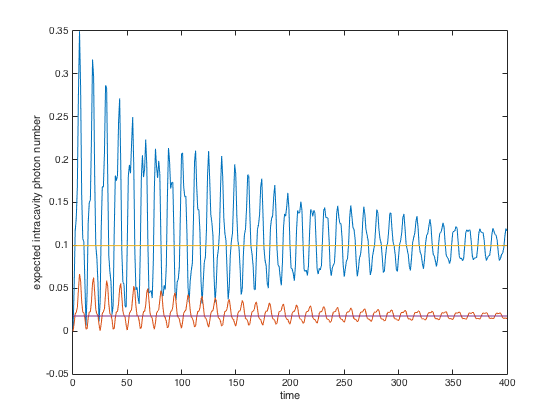
\includegraphics[width=1\textwidth]{Images/CriticalSlowing.png}
  \caption{Time Dependent Solutions with g=0.5, $\kappa$ = 0.01, blue line is (0.24, 1), red line is (0.1, 1)}\label{fig:CriticalSlowing}
\end{figure}

The plot containing evidence of critical slowing also contains a cut through the surface of \autocite[Figure 2]{Carmichael2015} for a given driving value (red squares.)

Figure 3b contains a surface and a contour plot of the steady state Q-function. In the contour plot the author highlights the upper half as indicative of the path of excitation (with a region of bimodality corresponding to the different excitation paths that are followed uniquely). The lower half of the plot corresponds to deexcitation.

These deexcitation fringes are clear in \ref{fig:Qbistabilities} where a spontaneous emission rate $ \gamma = \frac{\kappa}{2}$ connects the peaks of bistabilities in phases and amplitude. Given the interpretation of such bimodal quasi-probability functions in the zero detuning case as as having a probability peak for the occupation of each ladder, it is clear that spontaneous emission serves to induce ladder-switching.
\subsection{Spontaneous Emission}

The author investigates a limit of high photon numbers in which quantum fluctuations vanish and the mean field and exact theories coincide. He introduces what he calls the Maxwell-Bloch equations, the mean-field equations in the presence of spontaneous emission coupling to modes of the field other than the cavity fields. This shortens the Bloch vector in general, and thus the vector is no longer confined to the surface of the sphere.

The Maxwell-Bloch equations with spontaneous emission
\begin{align}
\frac{d \alpha}{dt} &= -(\kappa - i \Delta \omega)\alpha - ig \beta - i\Epsilon\label{eq:alphase}\\
\frac{d \beta}{dt} &= -(\frac{\gamma}{2}-i\Delta\omega)\beta+ig\alpha\zeta \label{eq:betase}\\
\frac{d\zeta}{dt} &= -\gamma (\zeta +1)+2ig(\alpha^*\beta-\alpha\beta^*) \label{eq:zetase}
\end{align}
In the steady state \cref{eq:alphase} becomes
\begin{align}
  \beta &= \frac{ig\alpha\zeta}{\frac{\gamma}{2}-i\Delta\omega}
\end{align}
from which in \cref{eq:zetase} in steady-state
\begin{align}
  0 &= -\gamma(\zeta+1)+2ig\frac{ig|\alpha|^2\zeta\frac{\gamma}{2}2}{\frac{\gamma^2}{4}+\Delta\omega^2} \\
  \implies \zeta &= \frac{1}{\frac{-2g^2|\alpha|^2}{\frac{\gamma^2}{4} +\Delta\omega^2}-1} \\
  &= \frac{1}{\frac{-2g^2|\alpha|^2 - \frac{\gamma^2}{4}-\Delta\omega^2}{\frac{\gamma^2}{4} +\Delta\omega^2}}
\end{align}
putting the above together yields
\begin{align}
  \beta &= \frac{ig\alpha\zeta}{\frac{\gamma}{2}-i\Delta\omega}\\
  &= \frac{ig\alpha}{\frac{(-2g^2|\alpha|^2-\frac{\gamma^2}{4}-\Delta\omega^2)(\frac{\gamma}{2}-i\Delta\omega)}{\frac{\gamma^2}{4}+\Delta\omega^2}}\\
  &= \frac{ig\alpha}{\frac{-2g^2|\alpha|^2-\frac{\gamma^2}{4}-\Delta\omega^2}{\frac{\gamma}{2}+i\Delta\omega^2}}\\
  &= \frac{ig\alpha(\frac{\gamma}{2}+i\Delta\omega)}{-2g^2|\alpha|^2-\frac{\gamma^2}{4}-\Delta\omega^2} \label{eq:betasolved}
\end{align}
\cref{eq:alphase} in the steady state with  \cref{eq:betasolved} becomes a condition for $\alpha$
\begin{align} % Here be weird bugs
0&=-(\kappa-i\Delta\omega)\alpha-ig\beta-i\Epsilon \\
0&=-{(\kappa-i\Delta\omega)}\alpha-g\frac{ig(\frac{\gamma}{2}+i\Delta\omega)}{-2g^2|\alpha|^2-\frac{\gamma^2}{4}-\Delta\omega^2}\alpha-i\Epsilon \\
\implies \alpha &= -i\Epsilon \frac{1}{\kappa-i\Delta\omega+\frac{g^2(\frac{\gamma}{2}+i\Delta\omega)}{\frac{\gamma^2}{4}+{\Delta\omega}^2+2g{|\alpha|}^2}}\label{eq:alphadetdiss}
\end{align}
Setting $\gamma$ and $\Delta\omega$ to zero, the condition becomes
\begin{equation}
  \alpha = -i\Epsilon\frac{1}{\kappa}
\end{equation}
which is notably not the same as \cref{eq:alphacondnotdet}.

\subsection{Difference between limits}
\autocite{Alsing1999}
  The presence of $\gamma$ in the Maxwell-Bloch Equations changes the asymptotic solutions, even if $\gamma$ is set to zero in these solutions. This is down to the breaking of the conservation law $4|\beta|^2 +\zeta^2 = 1$ by the presence of spontaneous emission. The solutions in the case that the limit is taken after steady state requirement is imposed are those of absorptive optical bistability. In the limit $\frac{\gamma}{\kappa} \rightarrow 0$ the rate at which these steady states becomes vanishingly small

\Cref{eq:alphadetdiss} is the classical solution for the steady state of a saturable two level transition, with a saturation photon number ($I \propto |\alpha|^2 \approx n_{sat}$) of $n_{sat} = \frac{\gamma^2}{8g^2}$. He takes $n_{sat} \rightarrow \infty$ as a definition of a `Thermodynamic limit'

